
\documentclass[a4paper]{llncs}

\usepackage{amssymb}
\setcounter{tocdepth}{3}
\usepackage{graphicx} 
\usepackage{natbib}
\usepackage[utf8]{inputenc}
\usepackage{varwidth}
\usepackage{here}
\usepackage{subfig}
\usepackage{url}
    
\newcommand{\keywords}[1]{\par\addvspace\baselineskip
\noindent\keywordname\enspace\ignorespaces#1}

\begin{document}

\mainmatter  % start of an individual contribution

% first the title is needed
\title{Das \\ Flussproblem}

% a short form should be given in case it is too long for the running head
\titlerunning{Das \\ Flussproblem}

% the name(s) of the author(s) follow(s) next
%
% NB: Chinese authors should write their first names(s) in front of
% their surnames. This ensures that the names appear correctly in
% the running heads and the author index.
%
\author{Jan Niklas Hollenbeck \\ und \\ Marco Leeske}
\institute{Hochschule Darmstadt}
\maketitle


\begin{abstract}

In dieser Arbeit wird das Problem zur Findung des maximalen
Flusses in Netzwerken beleuchtet.
Für diese Flussprobleme gibt es unterschiedliche Algorithmen, welche auf dem von Ford und Fulkerson basieren.
 Die vorhandene Literatur geht vor allem auf die theoretische Grundlage und Funktion der einzelnen Algorithmen ein,  aber bietet keinen zufriedenstellenden praktischen Vergleich zwischen diesen.
 Mit dieser Arbeit soll diese Lücke gefüllt werden und damit als Entscheidungshilfe für die Nutzung in der Praxis dienen.
Basierend auf dem Algorithmus von Ford und Fulkerson untersuchen wir die beiden optimierten Algorithmen von Edmonds und Karp sowie Dinic.
Ein Laufzeitvergleich wird mit Hilfe eines Programmes, welches anhand von Datensätzen die Algorithmen testet, realisiert.
Die Test Daten werden so gewählt, dass man die Unterschiede der Algorithmen erkennen, ihre Laufzeit praktisch testen und die jeweiligen Vor- und Nachteile der Algorithmen aufzeigen kann.
Anschließend werden die gesammelten Resultate der Laufzeittests verglichen,
wodurch der theoretische Vorteil des Algorithmus von Dinic praktisch nachgewiesen wird.
 Trotzdem bleibt die Frage, welcher Algorithmus bei unterschiedlichen Ausgangssituationen und Erwartungen den Vorzug erhält, dies kommt unter anderem auf den Anwendungsfall und persönliche Anforderungen an.

\end{abstract}

\section{Einleitung}
\label{Einleitung}

Auf den folgenden Seiten behandeln wir das Flussproblem, welches ein mathematisches Problem zur Findung des maximalen Flusses in Netzwerken beschreibt.
 Solche Probleme des realen Lebens, beispielsweise in Kanal- oder Verkehrsleitsystemen, werden als gerichtete Graphen modelliert und mittels Algorithmen gelöst.
 Zur Lösung des Flussproblems gibt es unterschiedliche Algorithmen, welche sich in Laufzeit und Funktion unterscheiden. Diese basieren auf dem Algorithmus von Ford und Fulkerson der den Grundstein für Weiterentwicklungen gelegt hat.
 Die vorhandene Literatur geht vor allem auf die theoretische Grundlage und Funktion der einzelnen Algorithmen ein,  aber bietet keinen zufriedenstellenden praktischen Vergleich zwischen diesen.
 Mit dieser Arbeit soll diese Lücke gefüllt werden und damit als Entscheidungshilfe für die Nutzung in der Praxis dienen.
Basierend auf dem Algorithmus von Ford und Fulkerson untersuchen wir die beiden optimierten Algorithmen von Edmond und Karp sowie Dinic.
Zwischen diesen werden Laufzeitvergleiche durchgeführt.
Diese werden mit Hilfe eines Programmes, welches anhand von Datensätzen die Algorithmen testet, realisiert.
Die Test Daten werden so gewählt, dass sie die Unterschiede der Algorithmen aufzeigen und man ihre Laufzeit praktisch prüfen kann.
Es werden die jeweiligen Vor- und Nachteile der Algorithmen aufgezeigt sowie die Implementierbarkeit geprüft. Anschließend werden die gesammelten Resultate der Laufzeittests verglichen.
Durch die Laufzeittests konnte der theoretische Vorteil des Algorithmus von Dinic praktisch nachgewiesen werden.
 Die Frage, welcher Algorithmus bei unterschiedlichen Ausgangssituationen und Erwartungen den Vorzug erhält, bleibt weiterhin bestehen, denn dies kommt unter anderem auf den Anwendungsfall und persönliche Anforderungen an.

\section{Einführung}
\label{Einfuehrung}

Das Flussproblem beschreibt ein mathematisches Problem in Netzwerken.\\
Flussprobleme können in Netzwerken mithilfe von Graphen modelliert und mittels Algorithmen gelöst werden. In den folgenden Zeilen werden die für diese Arbeit nötigen Voraussetzungen erläutert.

\subsection{Algorithmus}
\label{Algorithmus}

Ein Algorithmus ist eine konkrete und eindeutige Handlungsvorschrift, um Probleme oder Klassen von Problemen zu lösen. Beispiele für einfachste Algorithmen können Gebrauchsanweisungen, Rezepte, Bauanleitungen oder Hashfunktionen sein. Wir begegnen Algorithmen im täglichen Leben wie auch bei mathematischen oder informationstechnischen Anwendungen. Algorithmen sind keine neuzeitliche Erfindung, bereits im 9. Jahrhundert beschreibt der arabische Mathe\-matiker Al-Chwarismi (Namensgeber des Algorithmus) Algorithmen. Aus unserem heutigen Leben sind Algorithmen nicht mehr wegzudenken, Navigationssysteme zeigen uns den kürzesten Weg, Smartphones schlagen uns die nächsten zu schreibenden Worte vor oder unsere Texte werden auf Rechtschreibfehler geprüft. Das sind nur wenige von unzähligen Anwendungen, welche auf Algorithmen beruhen. Ein Algorithmus gibt die Vorgehensweise vor, wie Eingabedaten in Einzelschritten in Ausgabedaten umgewandelt werden, um ein bestimmtes Problem lösen zu können. Man spricht im Allgemeinen von Algorithmen, wenn folgende Eigenschaften erfüllt sind:\\

\begin{enumerate}
 
\item Ausführbarkeit\\
Jeder der Einzelschritte eines Algorithmus muss ausführbar sein.\\

\item Endlichkeit / Finitheit\\
Der Algorithmus bzw. dessen Beschreibung muss endlich sein.\\ 

\item Eindeutigkeit\\
Algorithmen dürfen keine widersprüchliche Beschreibung haben, diese muss eindeutig sein.\\

\item Terminierung\\
Ein Algorithmus muss nach endlich vielen Schritten ein Ergebnis liefern.\\

\item Determiniertheit\\
Bei gleichen Voraussetzungen muss ein Algorithmus stets zum gleichen Ergebnis kommen.\\

\item Determinismus\\
Der Folgeschritt muss immer bestimmt sein. Ein Algorithmus darf zu jedem Zeitpunkt nur maximal einen möglichen Schritt zu Fortsetzung haben.\\ \\
\citep{EigenschaftenVonAlgorithmen}
\end{enumerate} 

\subsection{Netzwerke}
\label{Netzwerke}
Hinter dem Begriff Netzwerk verbirgt sich ein System, das in unserem Fall, mittels Knoten und Kanten dargestellt wird. In dieser Arbeit werden Netz\-werke betrachtet, welche sich als mathematische Graphen modellieren lassen. Mithilfe solcher Netzwerke können Problemstellungen aus unserem Alltag so beschrieben werden, dass sie durch Anwendung geeigneter Algorithmen ver\-einfacht oder sogar gelöst werden können. Hier im speziellen werden wir uns dem $(s,t)$-Fluss in einem Netzwerk $(G,u,s,t)$ widmen, wobei  $G$ einem kanten\-bewerteten, gerichteten Graph mit den oberen Kapazitäten $u$ entspricht. Ein Knoten $s$ wird als Quelle, sowie ein Knoten $t$ als Senke bezeichnet. Die zwischen Quelle und Senke liegenden Knoten und Kanten können als Zwischenstationen aufgefasst werden. Überdies wird jeder Kante, einer Verbindung von zwei Knoten im Netzwerk, eine Kapazität $u$ ($>0$) zugewiesen. Sie gibt an, wie viel maximal durch die Kante fließen kann.\\ \\
\citep{Optimierungsmodell}

\subsection{Gerichtete Graphen}
\label{Graph}
Bei gerichteten, orientierten Graphen bzw. Digraphen werden die Kanten als Pfeile anstelle von Linien dargestellt. Die Pfeile beschreiben die Flussrichtung der Kanten wobei verdeutlicht wird, dass jede der Kanten nur in eine Richtung durchlaufen werden kann.\\

Der Graph selbst wird als
$G = (V,E)$ mit einer Menge V von Knoten und einer Menge
geordneter Knotenpaare $E \subseteq V x V$ von Kanten dargestellt.\\ \\
Kanten werden als 
$e = (a,b)$
mit $a$ als Start- und $b$ als Endknoten bezeichnet.
Zwei Kanten $e_{1}$ und $e_{2}$ mit 
$e_{1} = (a,b)$ und $e_{2} = (b,a)$
heißen gegenläufig oder antiparallel.\\ \\
Der Knoten $s$ zeigt den Startpunkt des Flusses. Alle durch das Netzwerk zu transportierenden Mengen starten ihren Fluss an diesem Knoten, mit dem Ziel, den Endknoten $t$ zu erreichen.\\ 

In Figure \ref{fig:Graph1} unter \ref{Graph} sieht man die Quelle auf der linken Seite, gekenn-zeichnet durch "$s$" und die Senke auf den rechten Seite dargestellt als "$t$" Des Weiteren sind die Kapazitäten "$u$" an jeder Kante angegeben. 

\begin{figure}[htbp] 
  \centering
     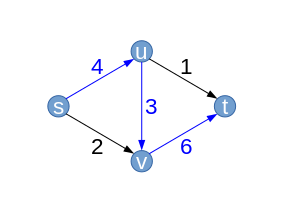
\includegraphics{graph1} 
  \caption{Bild eines ($s,t$)-Netzwerkes als gerichteter Graph \citep{GuN}}
  \label{fig:Graph1}
\end{figure}

\subsection{Algorithmus von Ford und Fulkerson}
\label{FuF}
Der Ford-Fulkerson Algorithmus ist der erste effiziente Algorithmus der in einem Netzwerk $(G,u,s,t)$ den maximalen Fluss $f$ errechnet. Der eigentliche Ablauf des Algorithmus ist sehr einfach: Man sucht einen beliebigen Pfad mit positiven Kapazitäten an allen Kanten von $s$ nach $t$ und bestimmt den maximal möglichen Fluss (geringste Kapazität auf dem Weg von $s$ nach $t$). Anschließend merkt man sich den Fluss, ändert die Kapazitäten an den Kanten entsprechend des ersten Durchlaufs ab und iteriert diesen Schritt bis kein Weg mehr zu finden ist. Die erhaltenen Flüsse werden aufaddiert und das Ergebnis entspricht dem maximalen Fluss.\\ \\Ablauf:\\ \\Input: Netzwerk $(G, u, s, t)$.\qquad Output: Maximaler Fluss $f$.\\ \\
Schritt 1: Setzen Sie $f(e) = 0$ für alle Kanten $e \subseteq E$.\\ \\Schritt 2: Bestimmen Sie $G^{f}$ und $u^{f}(e)$.\\ \\Schritt 3: Konstruieren Sie einen einfachen $(s, t)$-Weg $p$ in $G^{f}$. Falls keiner existiert:
STOPP.\\ \\Schritt 4: Verändern Sie den Fluss $f$ entlang des Wegs $p$ um $\gamma := min_{e \subseteq p}u^{f} (e)$.\\ \\Schritt 5: Gehen Sie zu Schritt 2\\ \\
\citep{GuN} \\ \\

\subsection{Breitensuche}
\label{Breitensuche}
Im Folgenden wird die Breitensuche behandelt, da sie zum verständinss der Algorithmen von Edmonds und Karp und Dinic benötigt wird.
Die Breitensuche (breadth first search) ist ein Suchalgorithmus für Graphen der zunächst alle von Ursprung ausgehenden Knoten Makiert, bevor die Folgeknoten untersucht werden Siehe Figur \ref{fig:Graph2}.
Mit ihm ist es möglich den Kürzesten Pfad zwischen Zwei Knoten zu finden.
In unserem Anwendungsfall wird die Quelle s als Startknoten definiert und von ihr ausgehend alle Pfade zur Senke gesucht. Der kürzeste wird dann zurück geliefert.
\begin{figure}[htbp] 
  \centering
     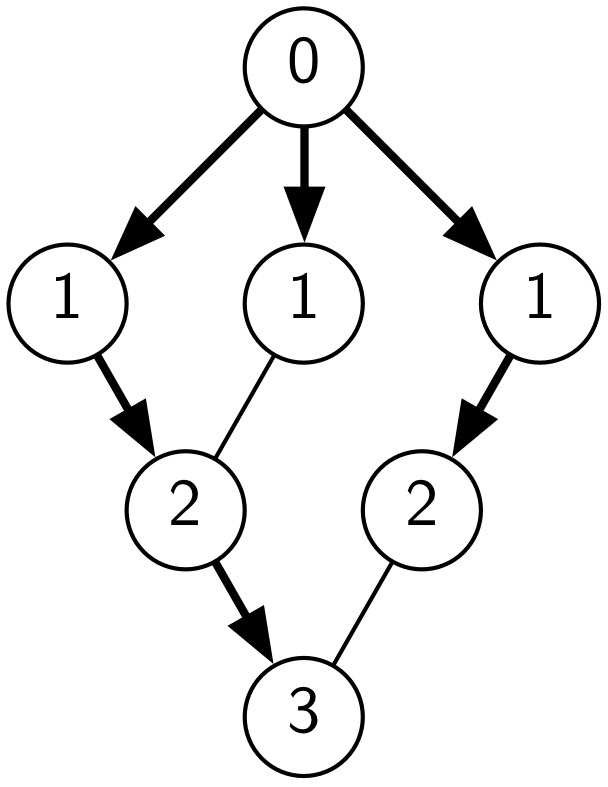
\includegraphics[scale=0.14]{BreitensucheGraph} 
  \caption{Die Ebenen werden nacheinander abgearbeitet, wenn Knoten bereits besucht wurden muss dieser nicht noch einmal makiert werden.}
  \label{fig:Graph2}
\end{figure}

\subsection{Algorithmus von Edmonds und Karp}
\label{EuK}
Der Algorithmus von Edmonds und Karp \ref{EuK} ist eine Weiterentwicklung des Ford und Fulkerson Algorithmus der 1972 publiziert wurde.
Er unterscheidet sich zum Ford Fulkerson durch seine zusätzliche Breitensuche \ref{Breitensuche},
welche immer den Kürzesten Weg von s nach t gemessen an der Anzahl von Kanten liefert. 
Entlang dieser wird der Fluss erhöt.
Im Vergelich zum ablauf in \ref{FuF} ändert sich Schritt Nr. 3 von einem einfachen $(s, t)$-Weg $p$ in $G^{f}$ zu dem Kürzesten.

\subsection{Algorithmus von Dinic}
\label{Dinic}
Dinic's Algorithmus ist dem von Edmonds und Karp sehr ähnlich. Auch hier wird im Gegensatz zu Ford und Fulkerson eine Breitensuche \ref{Breitensuche} durchgeführt. Der Unterschied zu Edmonds und Karp zeigt sich im Umgang mit den gefundenen Wegen. Bei Dinic wird nicht nur der kürzeste $(s, t)$-Weg $p$ in $G^{f}$ durchlaufen und berechnet, stattdessen werden große $(s, t)$-Flüsse aus mehreren kürzesten $(s, t)$-Wegen zusammengesetzt, anschließend abgearbeitet und der maximale Fluss ermittelt.

\section{Der Inhalt}
\label{Inhalt}
Wir führen im bezug auf die Mathematische Laufzeit eine Evaluierung der genannten Maximal-Fluss Algorithmen durch. Außerdem beschäftigen wir uns mit der praktischen implementierung der Algorithmen. Zuletzt wird ein Laufzeit Test der Algorithmen von Edmons und Karp sowie Dinic anhand von Testdaten durchgefürt.
Für die Laufzeit Test haben wir ein Java Programm an unser Bedürfnisse angepasst, welches den Maximalen Fluss errechnet. Für jede Berechnung wird die Zeit gemessen.
Da bei wenigen Durchläufen eine genaue Zeitmessung unmöglich ist werden jewails einhundert Messungen erstellt. Diese bestehen aus jewails einer Millionen Algorithmen Durchläufe von denen der Mittelwert errechnet wird.
Die Ergebnisse werden zur einfacheren Analyse in eine CSV Datei geschrieben.
Mit diesen Messungen wird das Verhältniss der Laufzeiten errechnet und auf Plausibilität geprüft.
Kriterien der Evaluierung, Vorstellung des Testaufbaus
\section{Experimente}
\label{Experimente}
Auflistung Test welche Daten benutzen wir und was wir damit erreichen wollen?
Unser test wurde mit jewails drei Testpaaren durchgeführt, die sich in ihrer Knotenanzahl unterscheiden.
Die einzelnen Paare unterscheiden sich jewails nur in der Anzahl ihrer Kanten.
Mit diesen test zeigen wir, dass der 
\subsection{Laufzeitvergleich}
Vergleich der Test Ergebnisse

\begin{figure}[H]
  \centering
     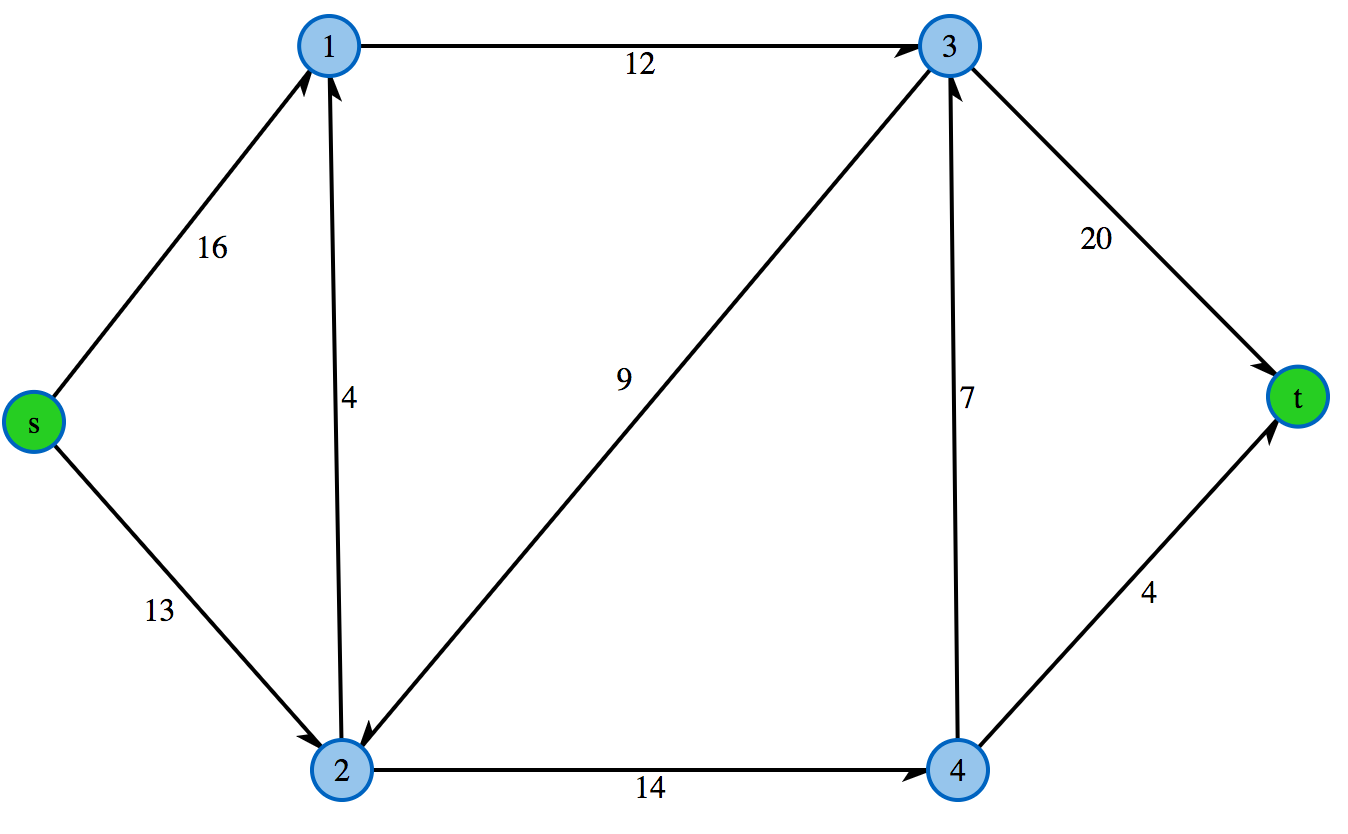
\includegraphics[scale=0.2]{testgraph1} 
  \caption{Testgraph1}
  \label{fig:testgraph1} 
  \centering
     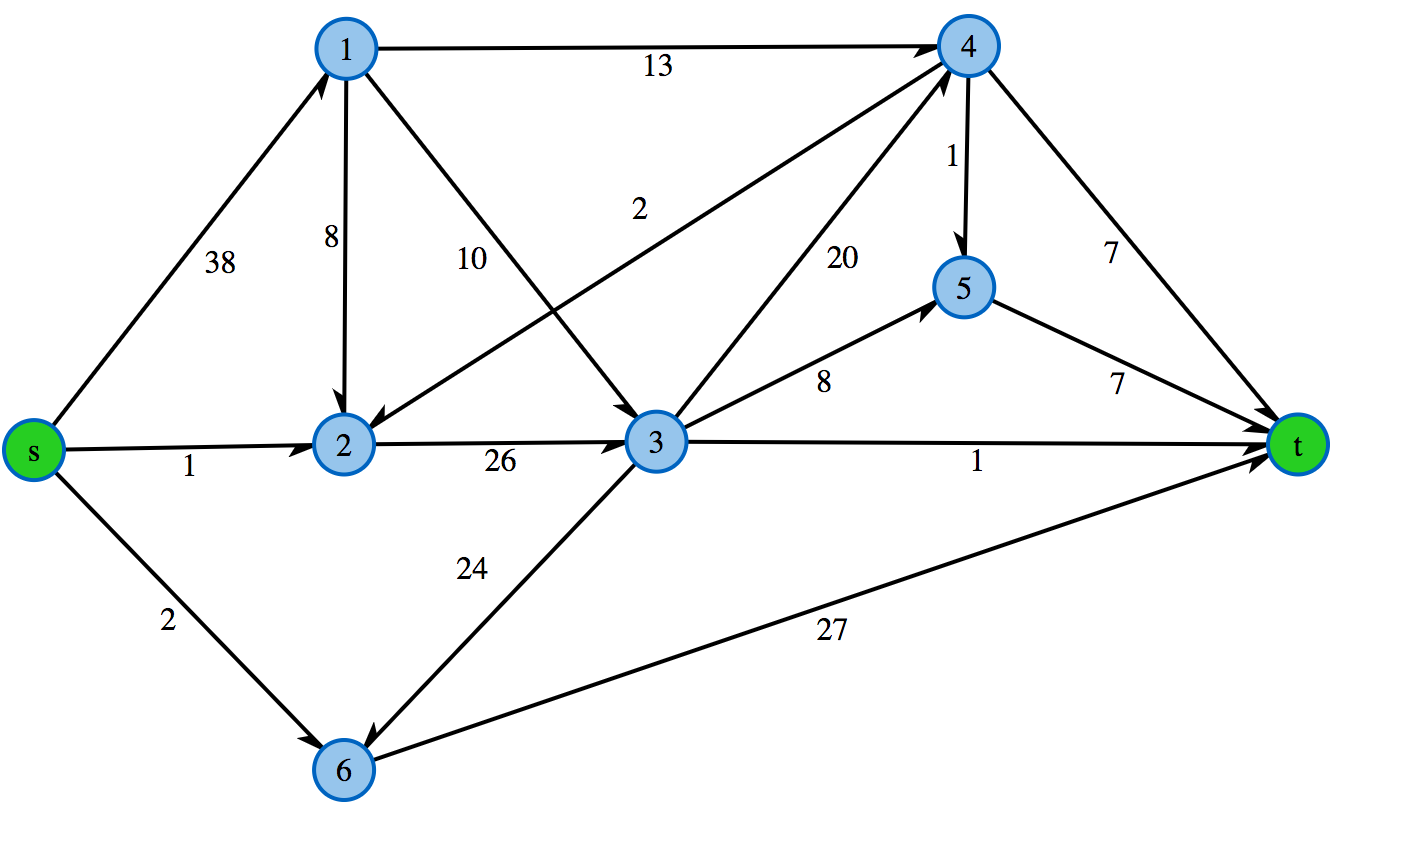
\includegraphics[scale=0.2]{testgraph2} 
  \caption{Testgraph2}
  \label{fig:testgraph2} 
  \centering
     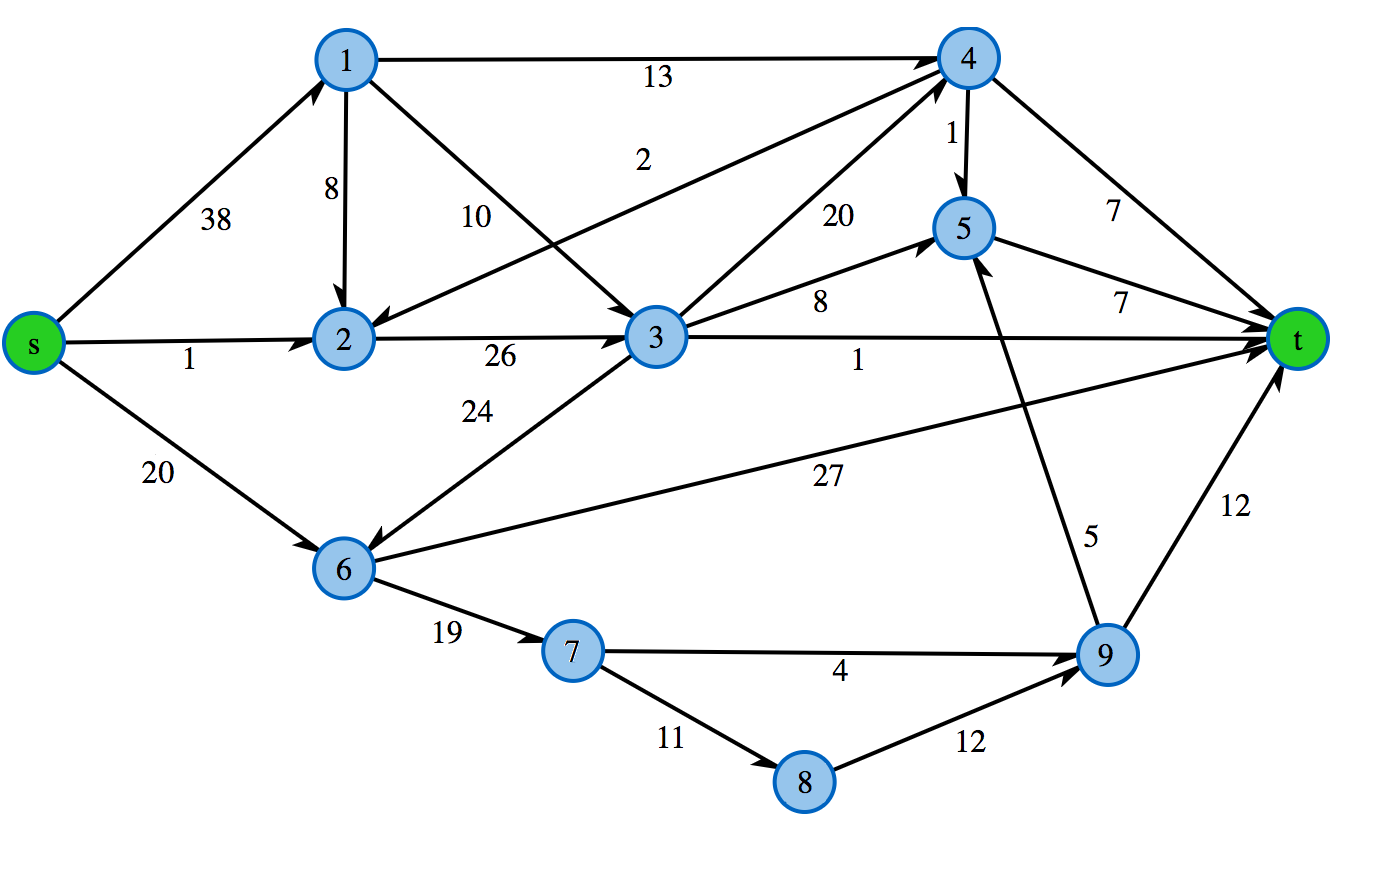
\includegraphics[scale=0.2]{testgraph3} 
  \caption{Testgraph3}
  \label{fig:testgraph3}
\end{figure}
\citep{FordFulkersonOnline}

\subsection{Anwendungszenarien der jeweiligen Algorithmen}
Die Ergebnisse also wann welcher anzuwenden ist

\section{Stand der Technik (Related Work)}
\label{Related Work}
Wie schon in der Einleitung \ref{Einleitung} erwähnt wurde, konnten wir keine, für uns befriedigende, vorangegangene Arbeit mit einem direkten, praktischen Laufzeitvergleich der beiden Algorithmen von Edmonds und Karp sowie dem von Dinic finden.

\section{Zusammenfassung}
\label{Zusammenfassung}
Anhand der unter \ref{Experimente} durchgeführten Laufzeittests, zeichnet sich der Vorteil des Dinic Algorithmus deutlich ab. Über je mehr Kanten ein Graph verfügt, desto vorteilhafter ist die Nutzung des Dinic Algorithmus. Fairerweise sollte aber gesagt sein, dass der Vorteil erst bei sehr großen Graphen zum tragen kommt. 
\subsection{Ausblick}
Erweiterung des Algorithmus von Dinic und Bottleneck erkennen.

\bibliography{quellen}
\bibliographystyle{plainnat} 

\end{document}
